\chapter{Nástroj Node-RED}
\label{ch:nastroj-node-red}

Node-RED je nástroj tvůrci popsaný jako \uv{Flow-based programming for the Internet of Things}, tedy nástroj založený na
programování na datovém toku určený pro IoT. Uživateli-programátorovi nabízí jednotlivé funkční bloky, jejichž vstupy a
výstupy lze vzájemně propojovat a vytvářet tak síť jakožto celek s požadovanými funkcemi. V roce 2013 jej představila
společnost IBM v rámci projektu JS Foundation pod licencí Apache 2.0. Nástroj vyžaduje běhové prostředí Node.js, tedy je
naimplementován v programovacím jazyke Javascript, od čehož se odvíjí i uživatelské rozšiřování.

\begin{figure}
    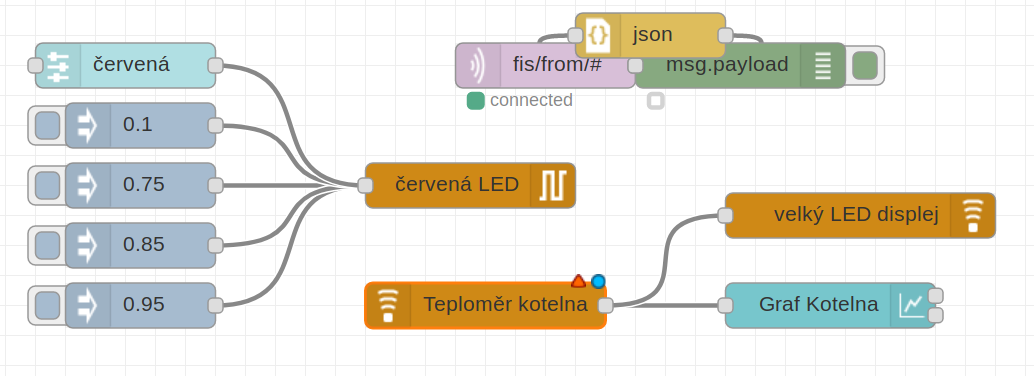
\includegraphics[width=\textwidth]{figures/node-red-example.png}
    \label{fig-node-red-example}
    \caption{Ukázka z Node-RED -- vstupy a výstupy jednotlivých bloků-uzlů spojené pro vzájemnou komunikaci.}
\end{figure}

\subsection{Programování datového toku}
Programovací paradigma založené na editaci datového toku bylo popsáno v již roce 1960 vědcem Jackem Dennisem. Jeho
principem je programování pomocí vytváření datových spojů mezi funkčními bloky.
\todo{Dataflow/flow based programming}
\blind{2}

\section{Principy použití Node-RED}

\todo{Pouziti, opensource}
Vnitřní architektura nástroje Node-RED je rozdělena na dva samostatné funkční bloky. V pohledu samotného běhu je
důležitější částí jádro provádějící veškeré datové operace nad samotným nadefinovaným modelem, zodpovědné za spouštění
jednotlivých uživatelských bloků, jejich synchronizaci a vzájemnou distribuci dat. Druhou částí je samotný vizuální
editor, který je ve výchozím nastavení dostupný pomocí protokolu HTTP. Pomocí něj je možné uživatelsky 


\subsection{Konfigurace systému}
\todo{Rozsiritelnost, config nodes}
\blind{2}

\missingfigure{Node-RED spojeni}

\section{Message Queuing Telemetry Transport}
\todo{MQTT}
\blind{2}